%%%%%%%%%%%%%%%%%%%%%%%%%%%%%%%%%%%%%%%%%%%%%%%%%%%%%%%%%%%%%%%%%%%%
%% I, the copyright holder of this work, release this work into the
%% public domain. This applies worldwide. In some countries this may
%% not be legally possible; if so: I grant anyone the right to use
%% this work for any purpose, without any conditions, unless such
%% conditions are required by law.
%%%%%%%%%%%%%%%%%%%%%%%%%%%%%%%%%%%%%%%%%%%%%%%%%%%%%%%%%%%%%%%%%%%%

\documentclass[
  digital, %% This option enables the default options for the
           %% digital version of a document. Replace with `printed`
           %% to enable the default options for the printed version
           %% of a document.
  twoside, %% This option enables double-sided typesetting. Use at
           %% least 120 g/m² paper to prevent show-through. Replace
           %% with `oneside` to use one-sided typesetting; use only
           %% if you don’t have access to a double-sided printer,
           %% or if one-sided typesetting is a formal requirement
           %% at your faculty.
  table,   %% This option causes the coloring of tables. Replace
           %% with `notable` to restore plain LaTeX tables.
  nolof,     %% This option prints the List of Figures. Replace with
           %% `nolof` to hide the List of Figures.
  nolot,     %% This option prints the List of Tables. Replace with
           %% `nolot` to hide the List of Tables.
  %% More options are listed in the user guide at
  %% <http://mirrors.ctan.org/macros/latex/contrib/fithesis/guide/mu/fi.pdf>.
]{fithesis3}
\usepackage{gensymb}
%% The following section sets up the locales used in the thesis.
\usepackage[resetfonts]{cmap} %% We need to load the T2A font encoding
\usepackage[T1,T2A]{fontenc}  %% to use the Cyrillic fonts with Russian texts.
\usepackage[
  main=slovak, %% By using `czech` or `slovak` as the main locale
                %% instead of `english`, you can typeset the thesis
                %% in either Czech or Slovak, respectively.
  english, german, russian, czech, slovak %% The additional keys allow
]{babel}        %% foreign texts to be typeset as follows:
%%
%%   \begin{otherlanguage}{german}  ... \end{otherlanguage}
%%   \begin{otherlanguage}{russian} ... \end{otherlanguage}
%%   \begin{otherlanguage}{czech}   ... \end{otherlanguage}
%%   \begin{otherlanguage}{slovak}  ... \end{otherlanguage}
%%
%% For non-Latin scripts, it may be necessary to load additional
%% fonts:
\usepackage{paratype}
\def\textrussian#1{{\usefont{T2A}{PTSerif-TLF}{m}{rm}#1}}
%%
%% The following section sets up the metadata of the thesis.
\thesissetup{
    date          = \the\year/\the\month/\the\day,
    university    = mu,
    faculty       = fi,
    type          = bc,
    author        = Henrieta Micheľová,
    gender        = f,
    advisor       = prof. RNDr. Ivana Černá{,} CSc.,
    title         = {Distribuované algoritmy pro rekonfiguraci platformy RoFI},
    TeXtitle      = {Distribuované algoritmy pro rekonfiguraci platformy RoFI},
    keywords      = {RoFI platforma, MPI, ...},
    TeXkeywords   = {RoFI platforma, MPI, \ldots},
    abstract      = {This is the abstract of my thesis, which can

                     span multiple paragraphs.},
    thanks        = {These are the acknowledgements for my thesis, which can

                     span multiple paragraphs.},
    bib           = example.bib,
}
\usepackage{makeidx}      %% The `makeidx` package contains
\makeindex                %% helper commands for index typesetting.
%% These additional packages are used within the document:
\usepackage{paralist} %% Compact list environments
\usepackage{amsmath}  %% Mathematics
\usepackage{amsthm}
\usepackage{amsfonts}
\usepackage{url}      %% Hyperlinks
\usepackage{markdown} %% Lightweight markup
\usepackage{listings} %% Source code highlighting
\lstset{
  basicstyle      = \ttfamily,%
  identifierstyle = \color{black},%
  keywordstyle    = \color{blue},%
  keywordstyle    = {[2]\color{cyan}},%
  keywordstyle    = {[3]\color{olive}},%
  stringstyle     = \color{teal},%
  commentstyle    = \itshape\color{magenta}}
\usepackage{floatrow} %% Putting captions above tables
\floatsetup[table]{capposition=top}
\begin{document}
\chapter*{Úvod}
\addcontentsline{toc}{chapter}{Úvod}

\chapter{Popis platformy RoFI}
RoFI je modulárna robotická platforma, ktorá vzniká na pôde Fakulty informatiky Masarykovej univerzity. Táto platforma zastrešuje vývoj modulárnych robotov a iného príslušenstva po ich hardvérovej, ale aj softvérovej stránke na rôznych úrovniach. 

Primárnym cieľom platformy RoFI je vytvorenie modulárnych robotov, ktoré je možné využiť k rôznym úlohám. Príkladom sú úlohy ako prechádzanie cez úzke priestory, prekonávanie prekážok a podobne. 

Ich dizajn je navrhovaný tak, aby bolo jednoduché a nie príliš finančne náročné ich fyzicky skonštruovať. Softvérové vybavenie pokrýva široké spektrum požiadaviek modulárnych robotov a je jednoduché na prácu aj menej skúseným užívateľom. Zároveň je platforma navrhnutá tak, aby bola ľahko rozšíriteľná o dodatočné periférie a pasívne prvky. 

Základnou jednotkou platformy RoFI sú moduly \cite{mrazekMasterThesis}, ktoré sú schopné sa vzájomne fyzicky prepojiť a zároveň medzi sebou komunikovať \cite{rofiCom}. Okrem toho sa každý modul dokáže pripojiť aj na pasívne prvky. 

Prepojenie viacerých modulov umožňuje vytvoriť tzv. RoFIbotov \cite{rofiWeb}, ktoré majú širšie spektrum funkcionalít ako samostatné moduly. Cieľom tejto práce je práve zamerať sa na RoFIbotov a ich schopnosť rekonfigurovať sa za špecifických podmienok (podrobnejší popis v kapitole \ref{sec:restrictions}). 

Pre účel tejto práce je v kapitole \ref{sec:moduleSpec} popísaná iba časť hardvérového vybavenia modulu a schopnosti prepájania modulov. Ďalšie rozšírenia, softvérové vybavenie a iné komponenty a návody sa nachádzajú na stránkach platformy \cite{rofiWeb}. 

\section{Formálna špecifikácia modulov}
\label{sec:moduleSpec}
Modul platformy RoFI bol navrhnutý tak, aby bol tzv. \textit{lattice type}\footnote{v preklade kryštálová mriežka - každý modul je umiestnený v pravidelnej 3D mriežke} a zároveň má vlastnosť \textit{grid-awareness}\footnote{pri pohybe modulu zasahuje modul do najnižšieho počtu polí mriežky}. V súčasnej dobe je platforma RoFI prispôsobená na mriežku o veľkosti 10\,cm. Podrobný popis vlastností sa nachádza v diplomovej práci \textit{RoFI – Distributed Metamorphic Robots} \cite{mrazekMasterThesis}. 

\begin{figure}[htbp]
    \centering
    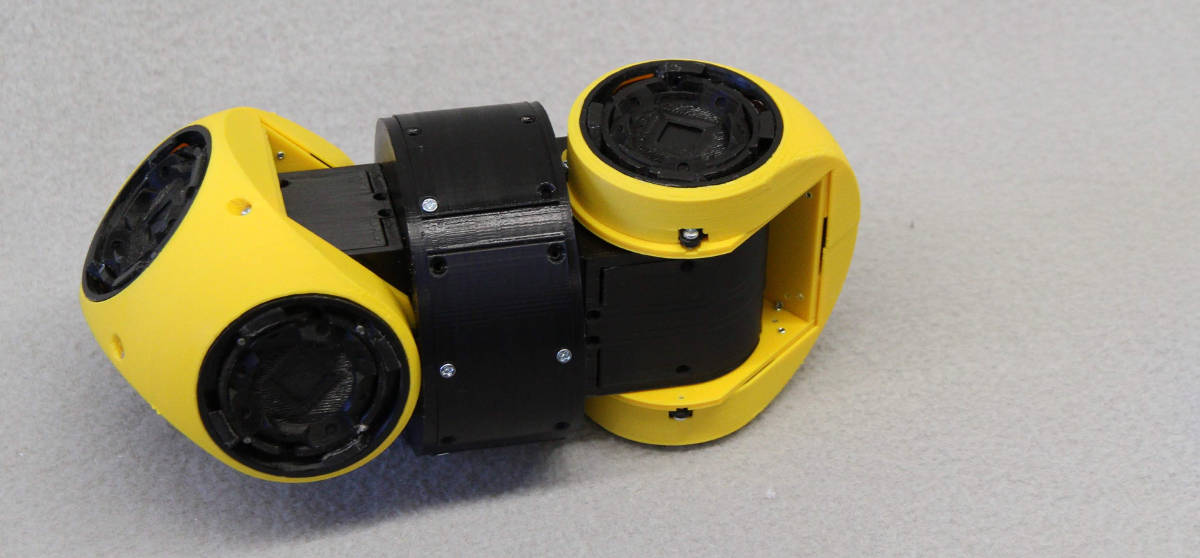
\includegraphics[width=0.6\textwidth]{pictures/module.jpg}
    \caption{//TODO popis+zdroj}
    \label{fig:module}
\end{figure}

Každý z modulov sa skladá z dvoch častí (\textit{side A} a \textit{side B}). Každá z nich sa delí na dve časti označené ako \textit{body} a \textit{shoe} (viď. obrázok \ref{fig:module_parts}). 

\begin{figure}[htbp]
    \centering
    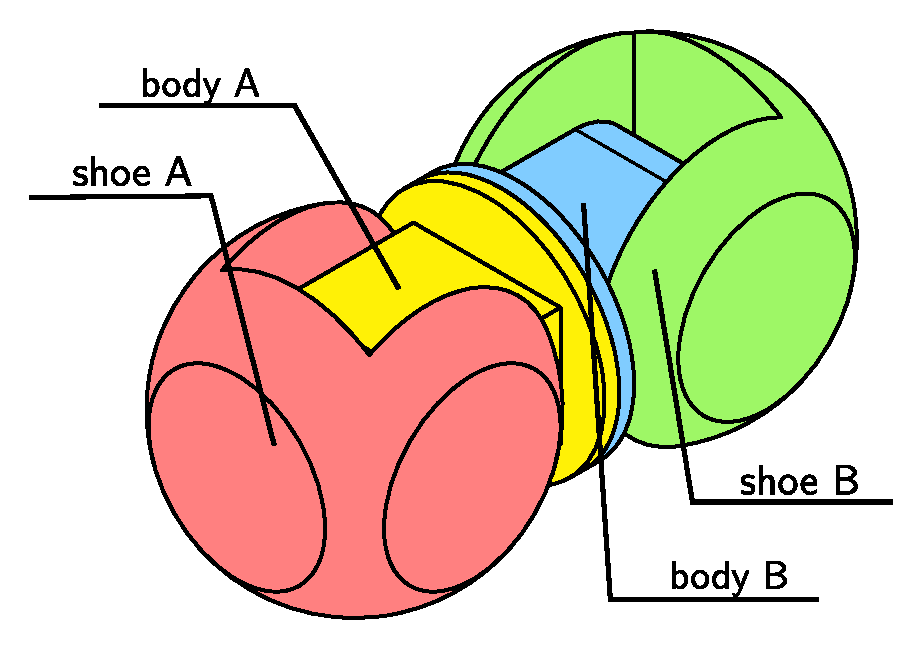
\includegraphics[width=0.6\textwidth]{pictures/module_parts.pdf}
    \caption{//TODO popis+zdroj}
    \label{fig:module_parts}
\end{figure}

Moduly majú schopnosť sa pohybovať, a to vďaka až trom stupňom voľnosti. Prvé dva z nich umožňujú pohybovať so \textit{shoe} časťou modulu. Konkrétne ide o pohyb okolo osí označovaných ako $\alpha$ a $\beta$  o uhol v rozsahu $\interval[{-90\degree, 90\degree}]$. Posledným stupňom voľnosti je pohyb okolo osi označovanej ako $\gamma$. Tento pohyb umožňuje otáčaním meniť vzájomnú polohu \textit{body} častí modulu a jeho rozsah je $\interval({-180\degree, 180\degree}]$. 

\begin{figure}[htbp]
    \centering
    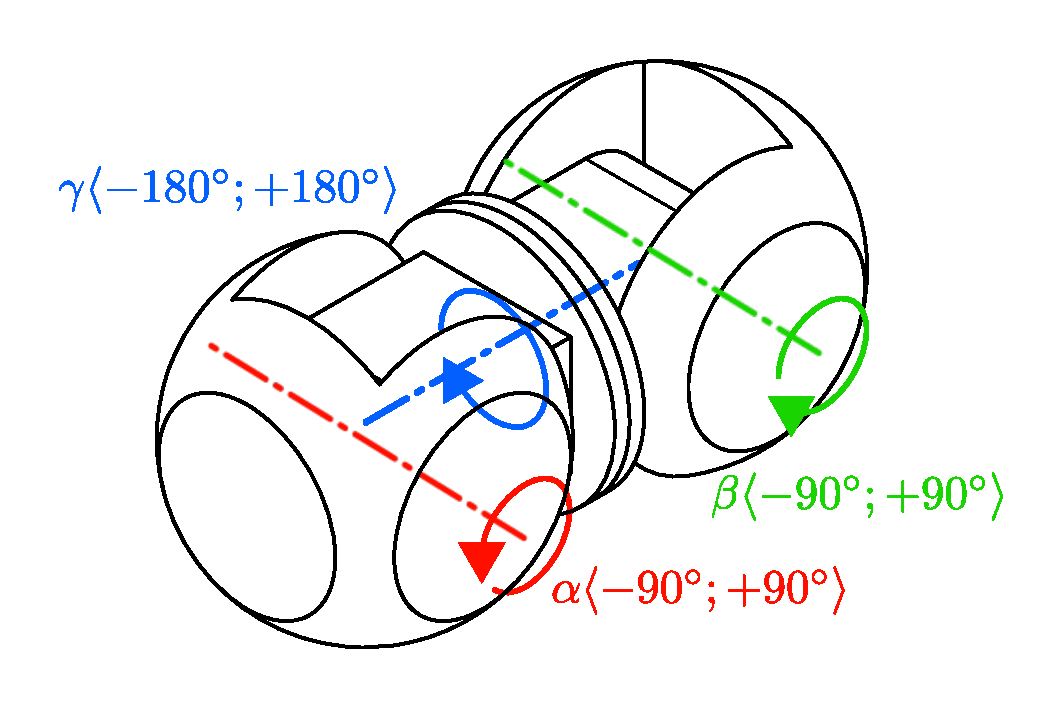
\includegraphics[width=0.6\textwidth]{pictures/module_angles.pdf}
    \caption{//TODO popis+zdroj}
    \label{fig:module_angle}
\end{figure}

Ako bolo spomenuté vyššie, tak každý modul má schopnosť pripojiť sa k iným modulom (a vytvoriť tak RoFIbotov) alebo k pasívnym prvkom pomocou dockov. Dockovací systém platformy RoFI je navrhnutý ako tzv. \textit{genderless}, čo umožňuje vzájomné spojenie ľubovoľných dvoch dockov. 

Každý modul obsahuje práve šesť dockov, ktoré sú rozmiestnené po tri na každej \textit{shoe} modulu. Dock je okrem svojej polohy na module definovaný aj orientačným vektorom (viď. obrázok \ref{fig:dock_desc}). Prepojenie je definované vzájomnou polohou orientačných vektorov dockov spojenia. 

\begin{figure}[htbp]
    \centering
    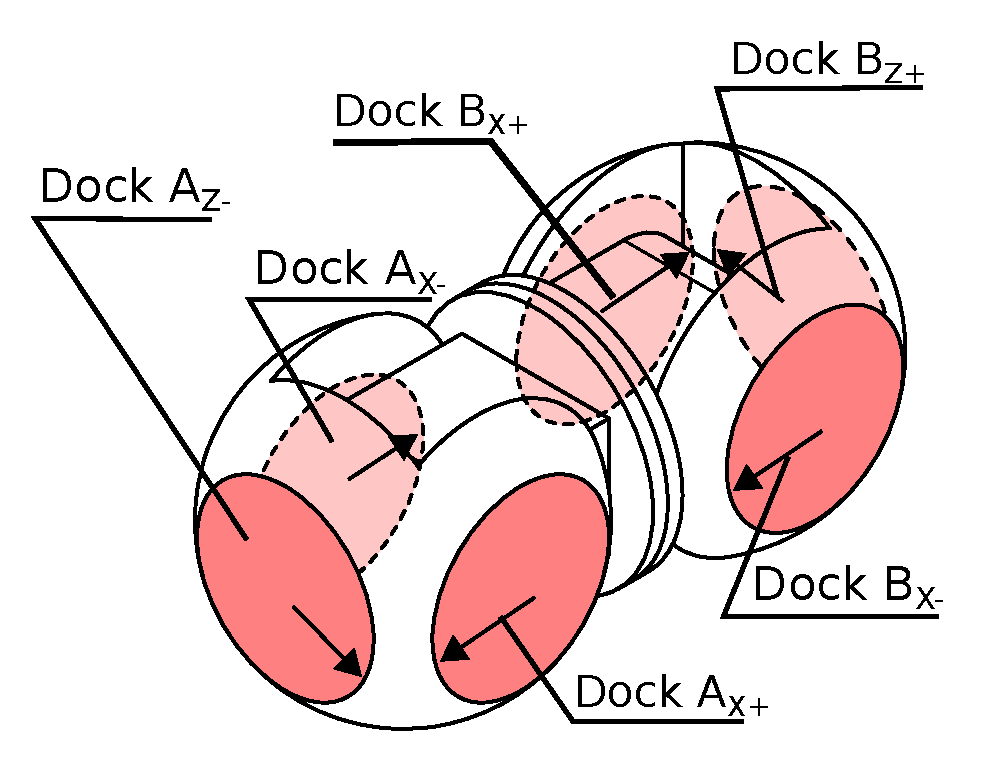
\includegraphics[width=0.6\textwidth]{pictures/dock_desc.pdf}
    \caption{//TODO popis+zdroj}
    \label{fig:dock_desc}
\end{figure}

Konštrukcia dockov dovoľuje ich prepojenie až v štyroch rôznych polohách. Vzájomná poloha orientačných vektorov dockov môže byť postupne $0\degree$, $90\degree$, $180\degree$ alebo $270\degree$ a tieto prepojenia sa označujú v tomto poradí ako \textit{north - N}, \textit{east - E}, \textit{south - S} a \textit{west - W} (viď. obrázok \ref{fig:dock_orientation}). 

\begin{figure}[htbp]
    \centering
    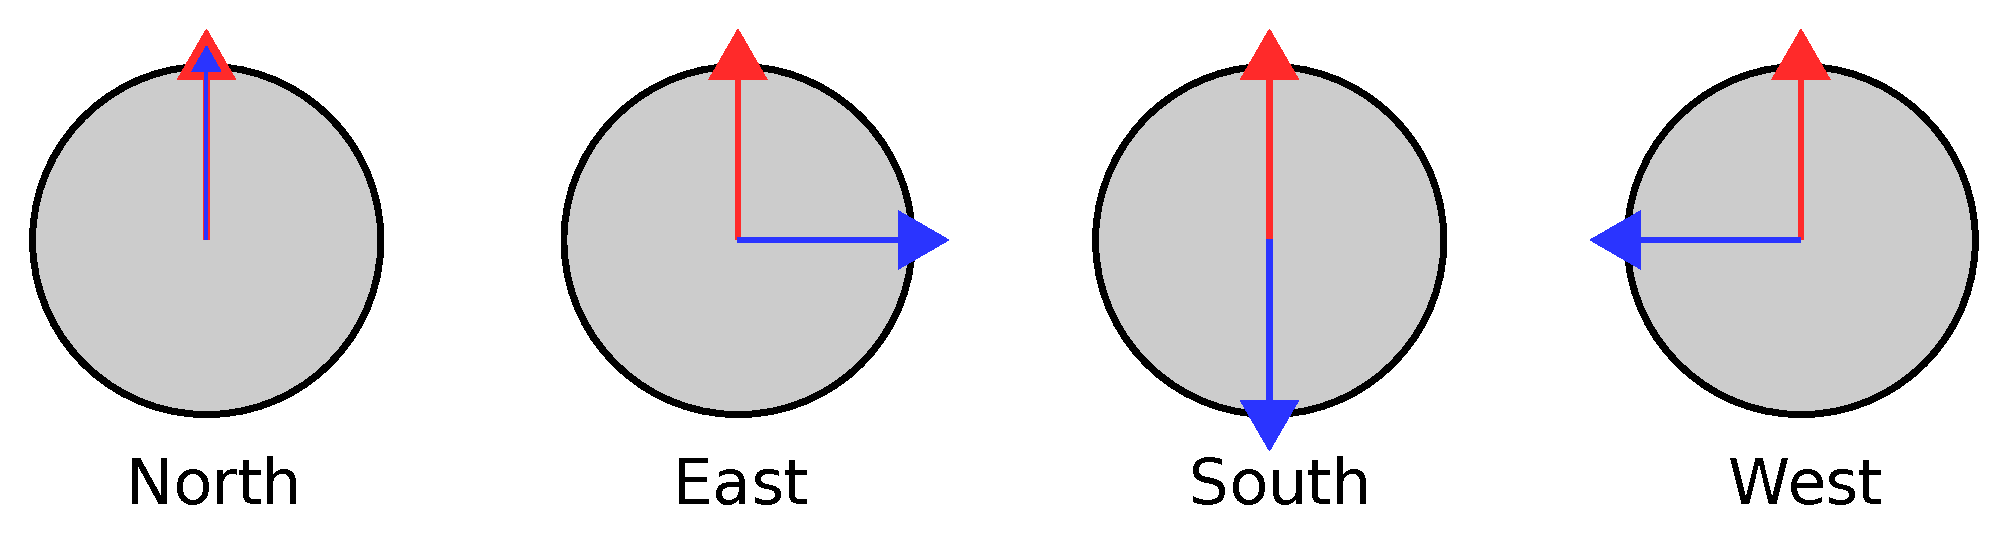
\includegraphics[width=0.6\textwidth]{pictures/dock_orientation.pdf}
    \caption{//TODO popis+zdroj}
    \label{fig:dock_orientation}
\end{figure}





\section{Obmedzenia pre môj problém}
\label{sec:restrictions}

\chapter{Vlastná práca}
\section{Formálna špecifikácia problému, vstupných a výstupných údajov - kompatibilita s vizualizérom}
\section{Popis ako funguje simulácia a využité knižnice}
\section{Popis navrhnutých a implementovaných algoritmov na rekonfiguráciu}
\subsection{Centralizovane-distribuovaný algoritmus}
\subsection{Distribuovaný algoritmus}

\chapter{Zhodnotenie a záver}
\section{Porovnanie algoritmov z pohľadu časovej a priestorovej zložitosti}
\section{Ukážkové konfigurácie a porovnanie rýchlostí ich výpočtov a prípadne rôznorodosti nájdených riešení}
\section{Popis, ktorý algoritmus a na aké konfigurácie a zmeny v rekonfiguráciách je viac vhodný}

  \printbibliography[heading=bibintoc] %% Print the bibliography.


\end{document}
